\section{Exoplanets \& Planetary Science}

\begin{sectionauthor}
    Madison Brady (The University of Chicago) \\
    Prof. Malena Rice (Yale University)
\end{sectionauthor}
\vspace{20pt}


\noindent Planets that are not in our own solar system are referred to as \textit{exoplanets}.  So far, we know of thousands of exoplanets in our universe.  From our observations, we are pretty confident that most stars host exoplanets.

\subsection{Types of Exoplanets}

There are several different types of exoplanets.  We usually describe exoplanets by comparing them to planets in the solar system.  However, there are some that are unlike anything in our solar system.


Small, rocky planets (also called \textit{terrestrial}) planets are usually compared to Earth.  They are made of similar stuff as the Earth (mostly rocky with some iron), though they can be more than ten times more massive (these larger rocky planets are called \textit{super-Earths}).  Rocky planets are extremely common in the universe, and tend to form close to their host stars, where the heat from the star prevents the buildup of gases or ices that would form less dense planets.  Due to their small sizes, rocky planets are very difficult to study.  This is disappointing, as rocky planets are the most likely places to host extrasolar life.

\begin{figure}[h!]
    \centering
    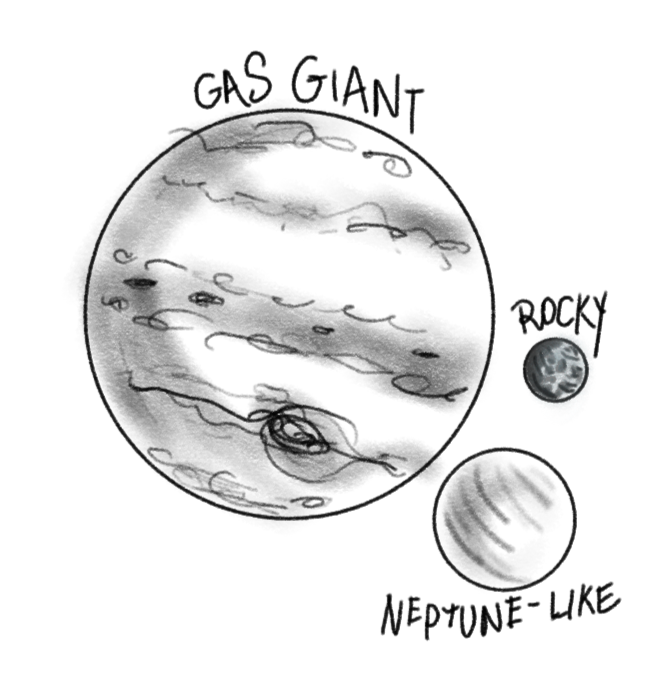
\includegraphics[width=0.4\linewidth]{img/planets.png}
    \caption{There are many different types of (exo)planets. We often use planets in our Solar System to help define exoplanet classification.}
    \label{fig:planets}
\end{figure}

Another common type of planet is the \textit{sub-Neptune}, named because they usually have sizes between that of Earth and Neptune.  These planets are less dense than rocky planets.  However, scientists don't know what they are made of.  They could be planets with rocky Earthlike cores and thick hydrogen/helium atmospheres, or planets with less dense ice-rich cores and much thinner atmospheres.  One hint as to their compositions comes from the well-known exoplanet radius gap- there are very few planets with radii in between sub-Neptunes and rocky terrestrial planets.  One explanation for this is that sub-Neptunes start out with thick atmospheres and then rapidly lose them (through either their own internal heat or that of the host star) to form rocky planets.  Another explanation is that planets have different compositions based upon where they form.  We need to study many more planets to know which explanation is true.

Giant planets are usually compared to Jupiter.  They are made of mostly hydrogen and helium, and can be up to ten times more massive than Jupiter. They are usually found around stars comparable to the sun or larger, as very low-mass stars frequently don't have enough mass around them to form large planets.  \textit{Hot Jupiters} are interesting because they are unlike anything in our solar system.  They are massive gas planets with orbital periods (or ``years") on the order of ten days or less.  These extreme planets likely formed far from the host star and migrated inwards.  Because hot Jupiters have large observable signatures and are relatively easy to find, hundreds are known in spite of their relatively low occurrence rate (around 1\% of sunlike stars).

\subsection{Observing Exoplanets}

Planets are very small and dim relative to stars.  As an example, the sun is about a hundred times larger in radius than the Earth and ten times larger than Jupiter.  This can make observing exoplanets directly very challenging.  A few common detection techniques are described in the sections below.

\subsubsection{Transits}
Exoplanets can eclipse their host stars, just as how our moon can sometimes eclipse the sun.  We can thus discover planets by studying the brightnesses of stars and looking out for dimming events.  The amount of light blocked by the planet is directly related to its size relative to the host star, so a transit event gives us a measurement of the planet’s size, which can be used to figure out what type of planet it is.

However, not every system has an orbit that causes eclipses, as the planet’s orbits need to line up so that the Earth, the planet, and the star fall on a straight line, which is a rare occurrence.  The further out the planet is from its star, the less likely it is to eclipse its host, so this technique tends to mostly discover planets on very short-period orbits, frequently with periods on the order of one to ten days.  This is much shorter than Mercury’s orbital period, which is 88 days.  Thus, it is difficult to look for planets like those in the solar system with this method.

It is (relatively) easy to design surveys to look for transiting planets with wide-field cameras that monitor many stars at once.  The \textit{Kepler} and \textit{TESS} missions are satellites that have discovered hundreds-to-thousands of exoplanets by studying large regions of the sky.  Transits are thus the most common exoplanet detection method.

With the launch of the James Webb Space Telescope (\textit{JWST}), we can also use exoplanet transits to study their atmospheres.  Molecules in an exoplanet’s atmosphere (such as water, methane, and carbon dioxide) can block different colors of light, so by studying the spectrum of light that passes through an exoplanet’s atmosphere as it transits its host star, we can learn about its contents.  We can use this information to learn about where planets form, how they evolve, and whether or not they are habitable.

\subsubsection{Radial Velocity}

One of the earliest methods of detecting exoplanets was the radial velocity method.  As a planet orbits around its host star, it will pull on the star with its own gravity, causing the star to complete its own (much smaller) orbit.  In general, all planets have some gravitational influence upon their star (even the Earth causes the Sun to move), and the strength of this influence will be based both upon the mass ratio of the planet to the star and the distance between the planet and the star.  We can measure the motion of the star directly using the \textit{Doppler effect}.


\begin{figure}[h!]
    \centering
    \includegraphics[width=0.5\linewidth]{img/Doppler.png}
    \caption{The Doppler effect caused by a moving source with respect to two observers, one \textit{in front} of the source, along the direction of motion, and one \textit{behind it}.}
    \label{fig:Doppler}
\end{figure}


The Doppler effect describes how waves change in frequency as the source moves.  As an example, consider the sound of a car driving past you and honking its horn.  As it is moving towards you, its horn sounds higher-pitched, which happens because the sound waves are compressed.  Meanwhile, after it passes you, the sound waves from the horn are stretched out, making it sound lower-pitched.  Something similar happens with light, which also has wave properties.  As something bright moves towards you, it will appear bluer, while it appears redder as it moves away. These differences in color are usually not something you can spot with the naked eye, but can be easily spotted by our telescopes.  

We can thus use the Doppler effect to study the motions of stars by looking at how they seem to change in color with time, looking bluer when they are moving towards us and redder when they are moving away.  With this information, we can learn about the mass and orbital period of any orbiting planets.  Understanding both the mass and radius of a planet is crucial when trying to figure out what it's made of, so planets are frequently studied with both the radial velocity and transit method (if possible).

While the radial velocity method allows us to study planets that don't transit their host stars, it tends to be more time-consuming.  Measuring the Doppler effect precisely typically requires much higher-powered telescopes than transit methods, and (unlike transits) it is difficult to measure the radial velocities of many stars simultaneously.  Thus, radial velocity surveys are typically used to more precisely characterize systems that were already identified as interesting through some other means (maybe they already have a transiting planet, maybe they are bright and nearby).


\subsubsection{Direct Imaging}
We can attempt to observe an exoplanet by just pointing a telescope at it and taking a picture.  While this may seem very straightforward, it is complicated by the fact that planets can be a million to a billion times dimmer than their host stars.  We thus cannot see the planets easily, much as how it’s difficult to see a firefly when it’s flying past a spotlight. 

One solution to this issue is to use \textit{coronagraphs}, which are astronomical instruments that block out the stellar light to allow us to search for any nearby planets.  However, it is difficult to fully block out all starlight, and these instruments thus have limitations that prevent us from directly imaging very small planets or planets that are very close to their host star.  However, we have directly imaged several large, young, bright planets on long-period orbits. A popular example is the HR 8799 system.

In addition, due to the wave nature of light, the light from a star and its nearby planet can blend together, making it impossible to distinguish them unless the planet has a very long-period orbit or the system is very close.  As this is an issue due to the nature of light (known as the \textit{diffraction limit}) and not due to any sort of instrumental limitations, there is no way to solve this problem besides using a telescope with a bigger mirror.  Even a ten-meter telescope (representative of the largest current-generation instruments) cannot directly image planets on Earthlike orbits outside of the solar neighborhood.

\subsection{Orbital Architectures}
Exoplanets orbit around their host stars in configurations, or ``architectures'', that can be examined to understand what types of planets are common, as well as how planets tend to be grouped into systems. The solar system includes four inner, rocky planets and four outer, gas giant planets, each on nearly circular orbits and with all planets orbiting in roughly the same direction that the Sun spins. In extrasolar systems, planets have been found in a wide range of configurations -- with neighboring planets of very different sizes, like in the WASP-47 system, or with planets orbiting sideways/backwards, like WASP-131 b.

The full orbital architecture of a planetary system is usually only partially known: that is, some planets are easier to find than others. Larger planets tend to produce the largest observable signatures, and planets that orbit in the same plane as their companions are often easier to find than planets that have larger orbital mutual inclinations. This means that the current census of known exoplanets is biased toward those with larger planets. While we don't yet have a conclusive answer regarding how common Earth-like planets are -- particularly since this occurrence rate is heavily dependent on what we would consider to be ``Earth-like'' -- it does appear that Jupiter analogues are relatively common.

One relatively well-characterized category of exoplanets is the hot Jupiters, which include a lone giant planet orbiting close to the host star. Hot Jupiters are often found on orbits that are not well-aligned with their host stars' spin axes, and they are generally not found with nearby planetary companions -- that is, hot Jupiters tend to be relatively lonely. 

\begin{figure}[h!]
    \centering
    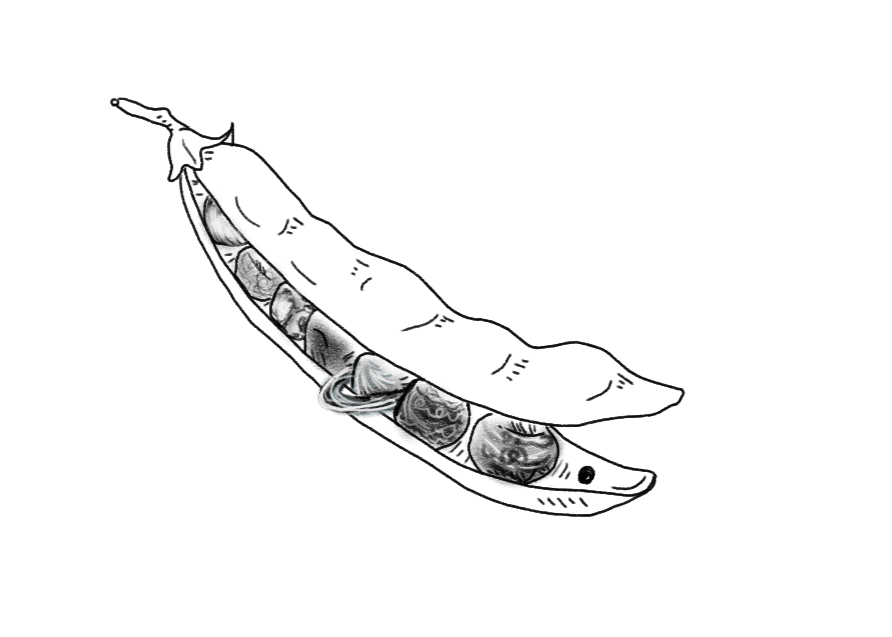
\includegraphics[width=0.5\linewidth]{img/peapod_planet.png}
    \caption{Planets aligned like peas in a pod.}
    \label{fig:peapod_planet}
\end{figure}

Another exciting and surprisingly common orbital architecture is the ``peas in a pod'' configuration, where multiple super-Earth or sub-Neptune sized exoplanets are found together with relatively equal spacings, masses, and radii. Peas-in-a-pod exoplanet systems somewhat resemble the inner solar system, but with much closer orbital spacings and with generally larger and more uniform planets (at least in terms of their masses and radii).
